%\chapter{Additional Materials}
\chapter{Appendices}% This will show as "Appendix A: Additional Materials"
%============================================================
\section*{Dataset Description and Provenance}
\label{app:dataset}

This study utilizes a large-scale, open-source Kiswahili speech corpus derived from community-contributed recordings. The dataset comprises short-form audio utterances paired with manually provided textual transcriptions and optional speaker metadata. Its primary objective is to support speech and language technology research for low-resource languages.

Each audio sample is accompanied by metadata attributes including speaker age group, gender, validation status, and community voting signals (upvotes/downvotes). All data were accessed and processed in compliance with the dataset’s licensing terms and ethical use guidelines. To ensure reproducibility, the dataset version, access date, and preprocessing scripts were fixed throughout all experiments.

% ============================================================
\section*{Data Cleaning and Quality Control}
\label{app:data_cleaning}

Exploratory analysis revealed several data quality challenges, including missing demographic attributes, transcription length variability, and audio artifacts such as background noise and extended silence.

The following preprocessing and cleaning steps were applied:

\begin{itemize}
    \item Removal of samples with missing, empty, or malformed transcriptions.
    \item Exclusion of audio clips exceeding predefined duration thresholds.
    \item Filtering of samples with low validation confidence.
    \item Standardization of text encoding, punctuation, and casing.
\end{itemize}

Figure~\ref{fig:missing_values} illustrates the distribution of missing metadata prior to cleaning.

\begin{figure}[h]
    \centering
    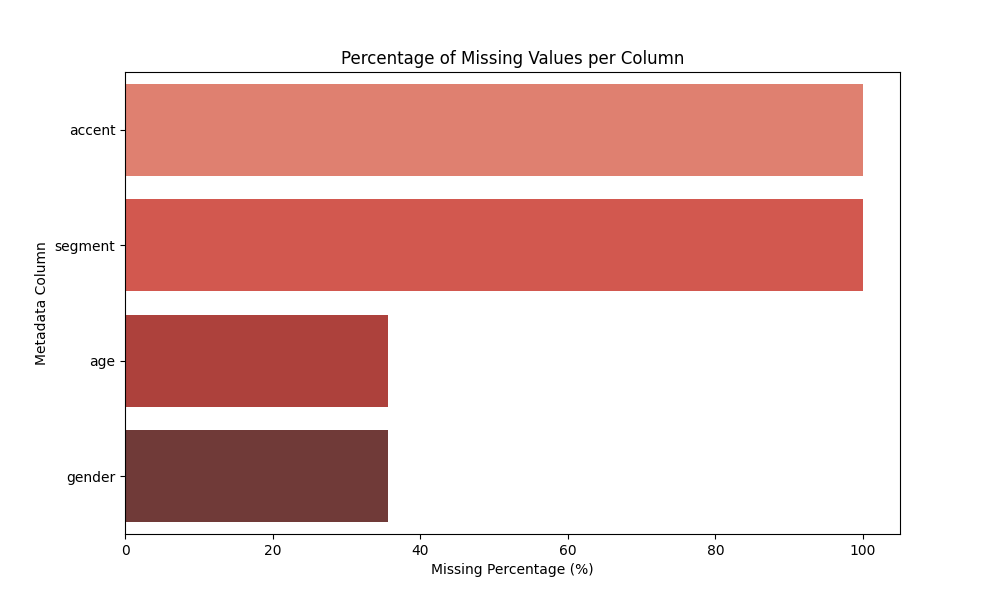
\includegraphics[width=0.8\linewidth]{images/missing_values.pdf}
    \caption{Visualization of missing values across metadata attributes prior to cleaning.}
    \label{fig:missing_values}
\end{figure}

% ============================================================
\section*{Demographic Distribution and Bias Assessment}
\label{app:demographics}

To assess representational bias, demographic distributions were examined across age and gender dimensions. Figures~\ref{fig:age_dist} and~\ref{fig:gender_dist} present the cleaned demographic distributions.

\begin{figure}[h]
    \centering
    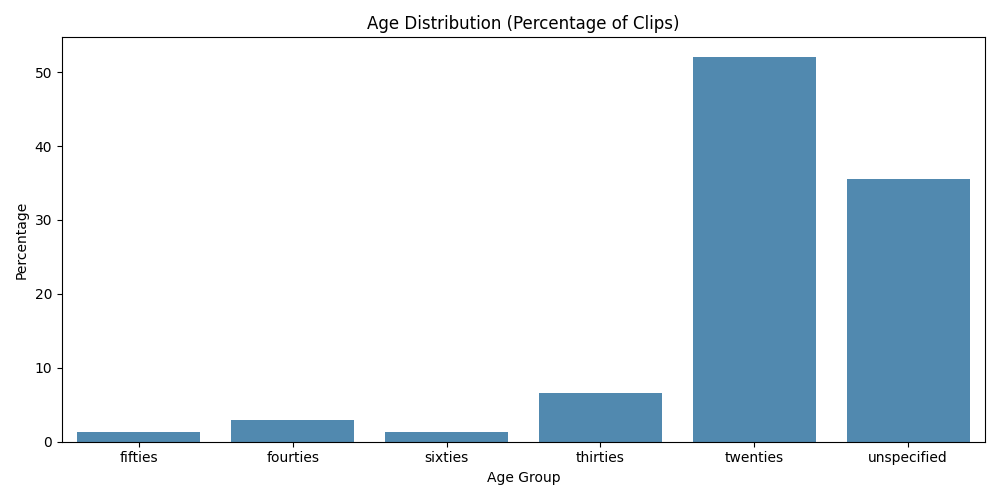
\includegraphics[width=0.75\linewidth]{images/age_distribution_cleaned.pdf}
    \caption{Age group distribution after dataset cleaning.}
    \label{fig:age_dist}
\end{figure}

\begin{figure}[h]
    \centering
    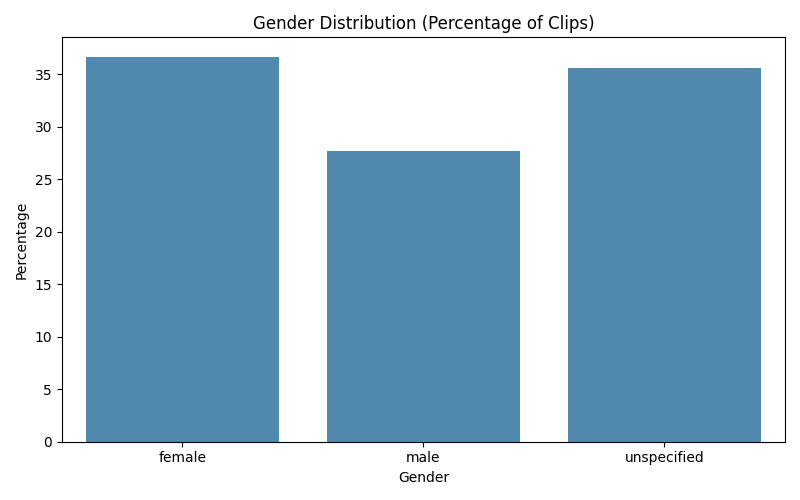
\includegraphics[width=0.75\linewidth]{images/gender_distribution_cleaned.pdf}
    \caption{Gender distribution after dataset cleaning.}
    \label{fig:gender_dist}
\end{figure}

The analysis reveals a demographic skew toward younger speakers and male contributors. These imbalances are acknowledged as potential sources of performance disparity in downstream ASR and sentiment inference tasks.

% ============================================================
\section*{Audio Preprocessing Pipeline}
\label{app:audio_preprocessing}

All audio samples were resampled to a uniform sampling rate of 16~kHz. Noise reduction and silence trimming were applied to improve signal quality prior to transcription. Spectral gating was used to attenuate stationary background noise.

The noise reduction process is expressed as:

\begin{equation}
y(t) = x(t) - \hat{n}(t)
\end{equation}

where $x(t)$ represents the original signal and $\hat{n}(t)$ denotes the estimated noise component.

Figure~\ref{fig:noise_spec} illustrates the impact of noise reduction on the signal spectrogram.

\begin{figure}[h]
    \centering
    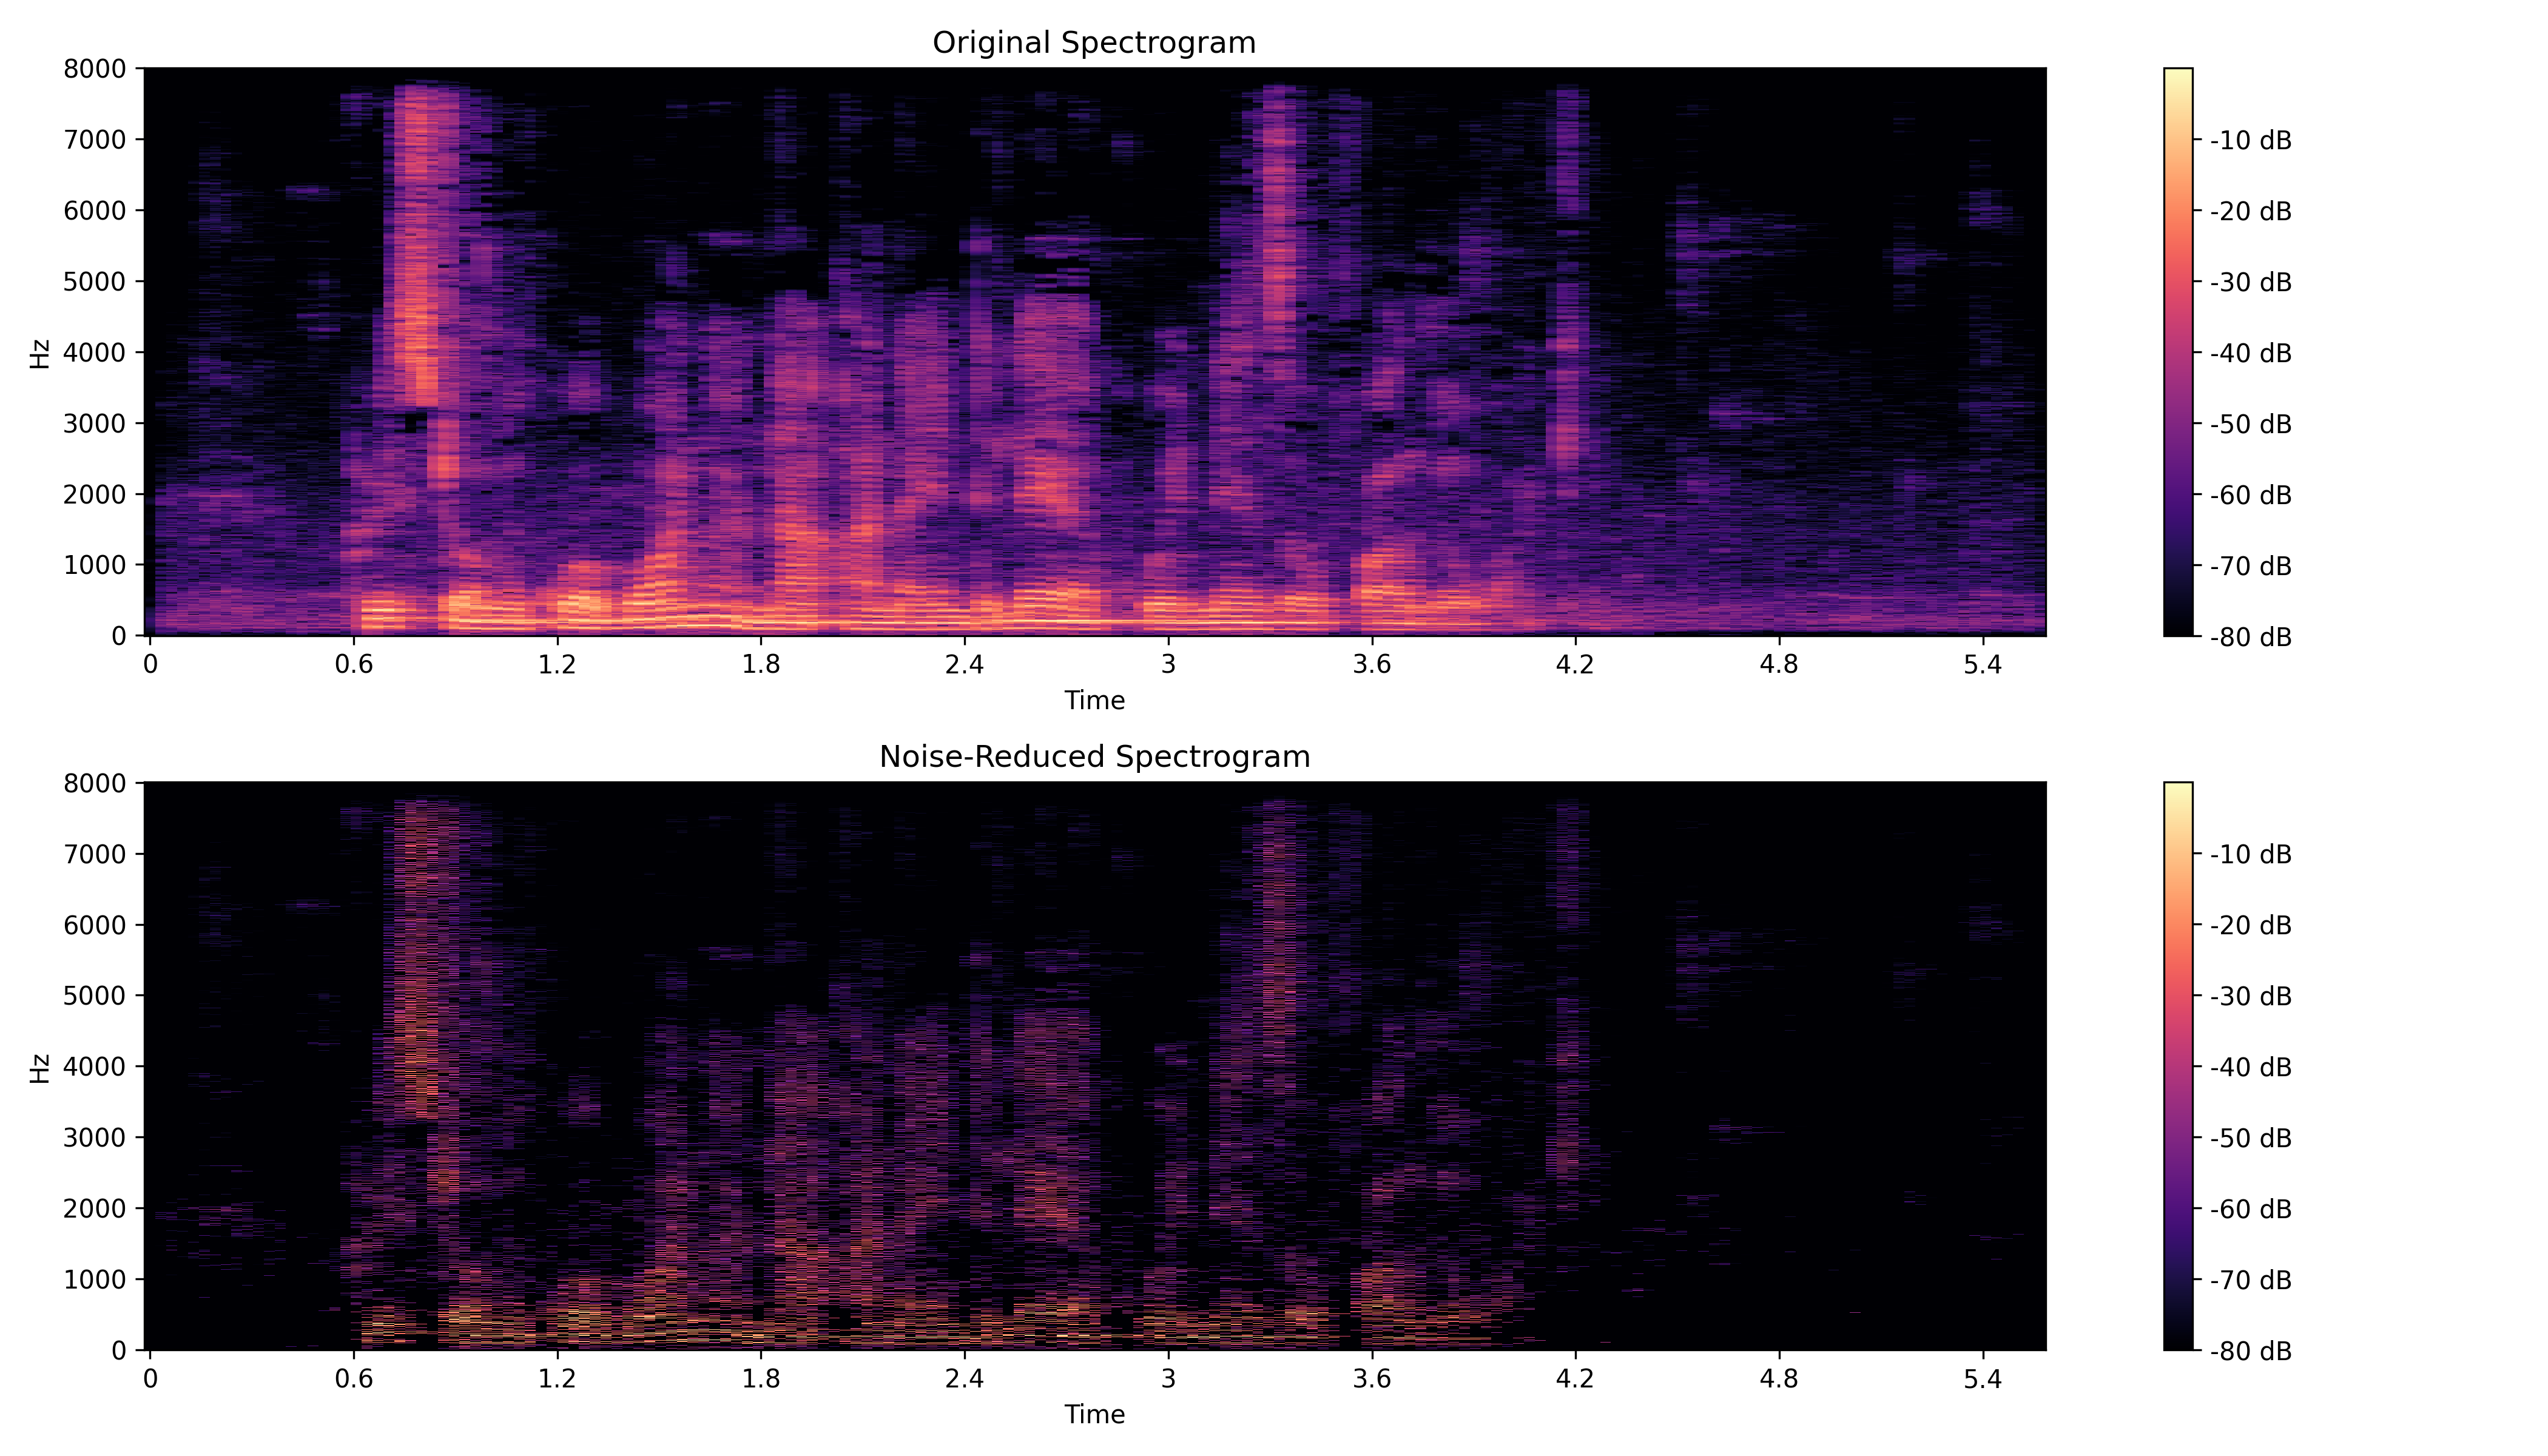
\includegraphics[width=0.8\linewidth]{images/noise_reduction_spectrogram.pdf}
    \caption{Spectrogram comparison before and after noise reduction.}
    \label{fig:noise_spec}
\end{figure}

% ============================================================
\section*{Automatic Speech Recognition Model Configuration}
\label{app:asr_config}

The ASR component employs a transformer-based architecture pretrained on multilingual speech corpora. The model performs end-to-end speech-to-text inference without explicit phoneme modeling.

Key configuration parameters are summarized in Table~\ref{tab:asr_params}.

\begin{table}[h]
\centering
\caption{ASR model configuration parameters.}
\label{tab:asr_params}
\begin{tabular}{ll}
\hline
Parameter & Value \\
\hline
Architecture & Transformer-based (Wav2Vec2/Whisper) \\
Sampling Rate & 16 kHz \\
Batch Size & 8 \\
Decoding Strategy & Greedy Decoding \\
Language & Kiswahili \\
\hline
\end{tabular}
\end{table}

% ============================================================
\section*{ASR Evaluation Metrics and Error Analysis}
\label{app:asr_eval}

Transcription quality was evaluated using Word Error Rate (WER), defined as:

\begin{equation}
\text{WER} = \frac{S + D + I}{N}
\end{equation}

where $S$, $D$, and $I$ represent substitution, deletion, and insertion errors respectively, and $N$ is the number of reference words.

Error analysis revealed that substitution errors dominated, particularly in code-switched utterances, named entities, and region-specific lexical forms.

% ============================================================
\section*{Text Processing and Linguistic Statistics}
\label{app:text_processing}

Prior to downstream NLP tasks, transcripts were normalized through lowercasing, punctuation removal, tokenization, and stopword filtering. Sentence and word length statistics are shown in Figure~\ref{fig:text_len}.

\begin{figure}[h]
    \centering
    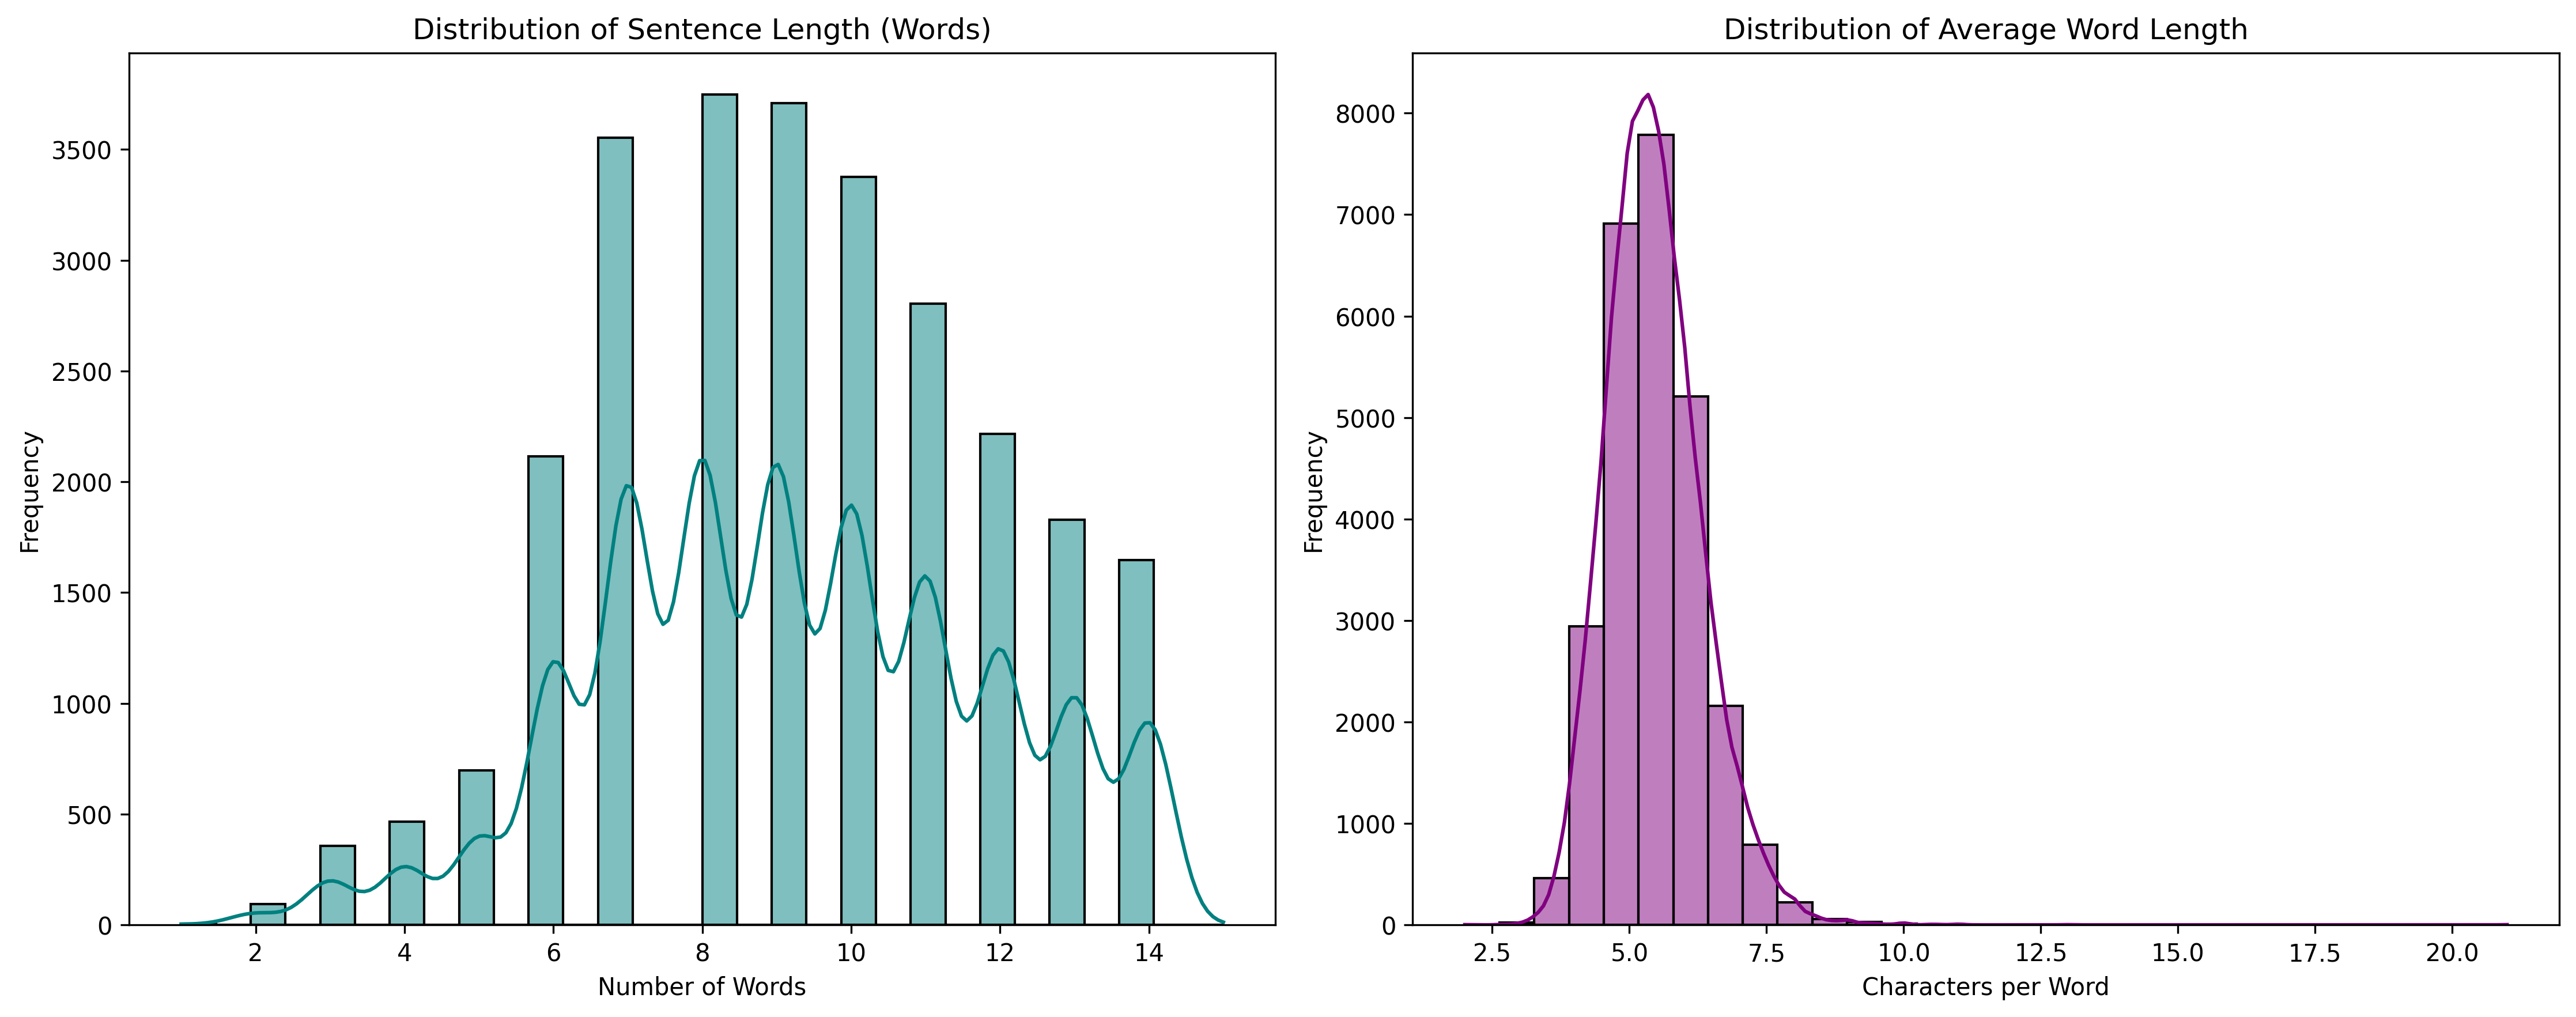
\includegraphics[width=0.75\linewidth]{images/sentence_and_word_length_distributions.pdf}
    \caption{Sentence and word length distributions across transcripts.}
    \label{fig:text_len}
\end{figure}

% ============================================================
% =========================
% APPENDIX: LINGUISTIC RESOURCES
% =========================
\section*{Custom Kiswahili Stopword Inventory}
\label{app:stopwords}

\subsection*{Motivation for Custom Swahili Stopword Design}

Natural Language Processing (NLP) tasks in low-resource languages such as Kiswahili require carefully curated linguistic resources. Kiswahili is a morphologically rich and agglutinative language, characterized by complex verb morphology, extensive agreement markers, and frequent use of functional particles. As a result, generic or English-oriented stopword lists are inadequate and may either fail to suppress high-frequency grammatical noise or inadvertently remove semantically meaningful units.

To address this challenge, this study developed a \textbf{custom Swahili stopword list} through iterative corpus inspection, exploratory data analysis, and linguistic validation. The goal was to reduce lexical noise while preserving semantic integrity across downstream tasks such as sentiment analysis, topic exploration, and text summarization.

\subsection*{Role of Stopwords in the Processing Pipeline}

The curated stopword list was applied consistently during the text preprocessing stage of the pipeline. Specifically, it was used in:
\begin{itemize}
    \item Token filtering prior to frequency-based analysis (unigrams and bigrams).
    \item Generation of word clouds and keyword visualizations.
    \item Preprocessing steps for sentiment analysis and abstractive summarization.
\end{itemize}

This ensured that high-frequency grammatical tokens did not dominate analytical outputs, thereby improving interpretability and robustness of the results.

\subsection*{Final Swahili Stopword Inventory}

The final stopword inventory was organized into linguistically meaningful categories, including conjunctions, pronouns, demonstratives, interrogatives, auxiliary verbs, discourse markers, and morphological verb prefixes. The list below represents the complete stopword set used throughout the experiments.

\textbf{Basic Functional Words and Pronouns}
\begin{verbatim}
na, lakini, ingawa, ingawaje, hadi, hata, kama, ilhali,
ya, yake, yao, yangu, yetu, yenu,
mimi, sisi, wewe, nyinyi, yeye, wao,
ni, sio, siye, ndio, hapana, au, ama
\end{verbatim}

\textbf{Demonstratives and Determiners}
\begin{verbatim}
hii, hizi, ile, zile, huyo, hao, hili, hilo,
haya, hayo, hiki, hiki, vile, vyote, lote, wote
\end{verbatim}

\textbf{Prepositions and Locative Expressions}
\begin{verbatim}
kwa, katika, kwenye, katikati, miongoni, kabla, baada,
nje, ndani, juu, chini, karibu, mbali
\end{verbatim}

\textbf{Conjunctions and Linking Expressions}
\begin{verbatim}
kwa sababu, kwa hiyo, hivyo basi, hata hivyo,
kwani, ila, bali, isipokuwa, ikiwa
\end{verbatim}

\textbf{Interrogatives}
\begin{verbatim}
nani, nini, gani, wapi, lini, vipi, kwanini, je
\end{verbatim}

\textbf{Temporal Adverbs}
\begin{verbatim}
leo, jana, kesho, sasa, baadaye, tangu, mara,
hivi karibuni, hapo awali
\end{verbatim}

\textbf{Manner and Emphasis Adverbs}
\begin{verbatim}
kabisa, hasa, pia, zaidi, pengine, huenda,
hakika, bila shaka
\end{verbatim}

\textbf{Verb Prefixes and Morphological Markers}
\begin{verbatim}
ku, ni, u, a, tu, m, wa, li, ya, ki, vi,
ame, ali, ata, ana, wana, wame, wali,
nime, tume, mme
\end{verbatim}

\textbf{Auxiliary and Light Verbs}
\begin{verbatim}
kuwa, kuwa na, kuwepo, kufanya, kuendelea,
kuonekana, huwa, kuna
\end{verbatim}

\textbf{Discourse Markers}
\begin{verbatim}
yaani, mfano, maana, kwa maana ya, hivyo
\end{verbatim}

\textbf{Generic Nouns and Fillers}
\begin{verbatim}
kitu, vitu, jambo, mambo, watu
\end{verbatim}

\textbf{Single-Character Tokens}
\begin{verbatim}
a, b, c, d, e, f, g, h, i, j, k, l, m,
n, o, p, q, r, s, t, u, v, w, x, y, z
\end{verbatim}

\subsection*{Implications for Model Performance}

The use of a linguistically informed stopword list contributed to:
\begin{itemize}
    \item Improved clarity in lexical frequency analysis and word cloud visualizations.
    \item Reduced noise in sentiment polarity estimation.
    \item More coherent and content-focused summaries.
\end{itemize}

However, it is acknowledged that aggressive stopword removal in morphologically rich languages can risk information loss. Future work may explore adaptive or context-aware stopword filtering to further improve downstream performance.

%============================================================
\section*{Sentiment Analysis Model and Outputs}
\label{app:sentiment}

Sentiment classification was conducted using a transformer-based multilingual DistilBERT model fine-tuned for polarity detection. Given logits $z$, class probabilities were computed using the softmax function:

\begin{equation}
P(y_i) = \frac{e^{z_i}}{\sum_{j} e^{z_j}}
\end{equation}

Confidence scores correspond to the maximum predicted class probability. Figure~\ref{fig:sentiment_dist} presents the distribution of predicted sentiment labels.

\begin{figure}[h]
    \centering
    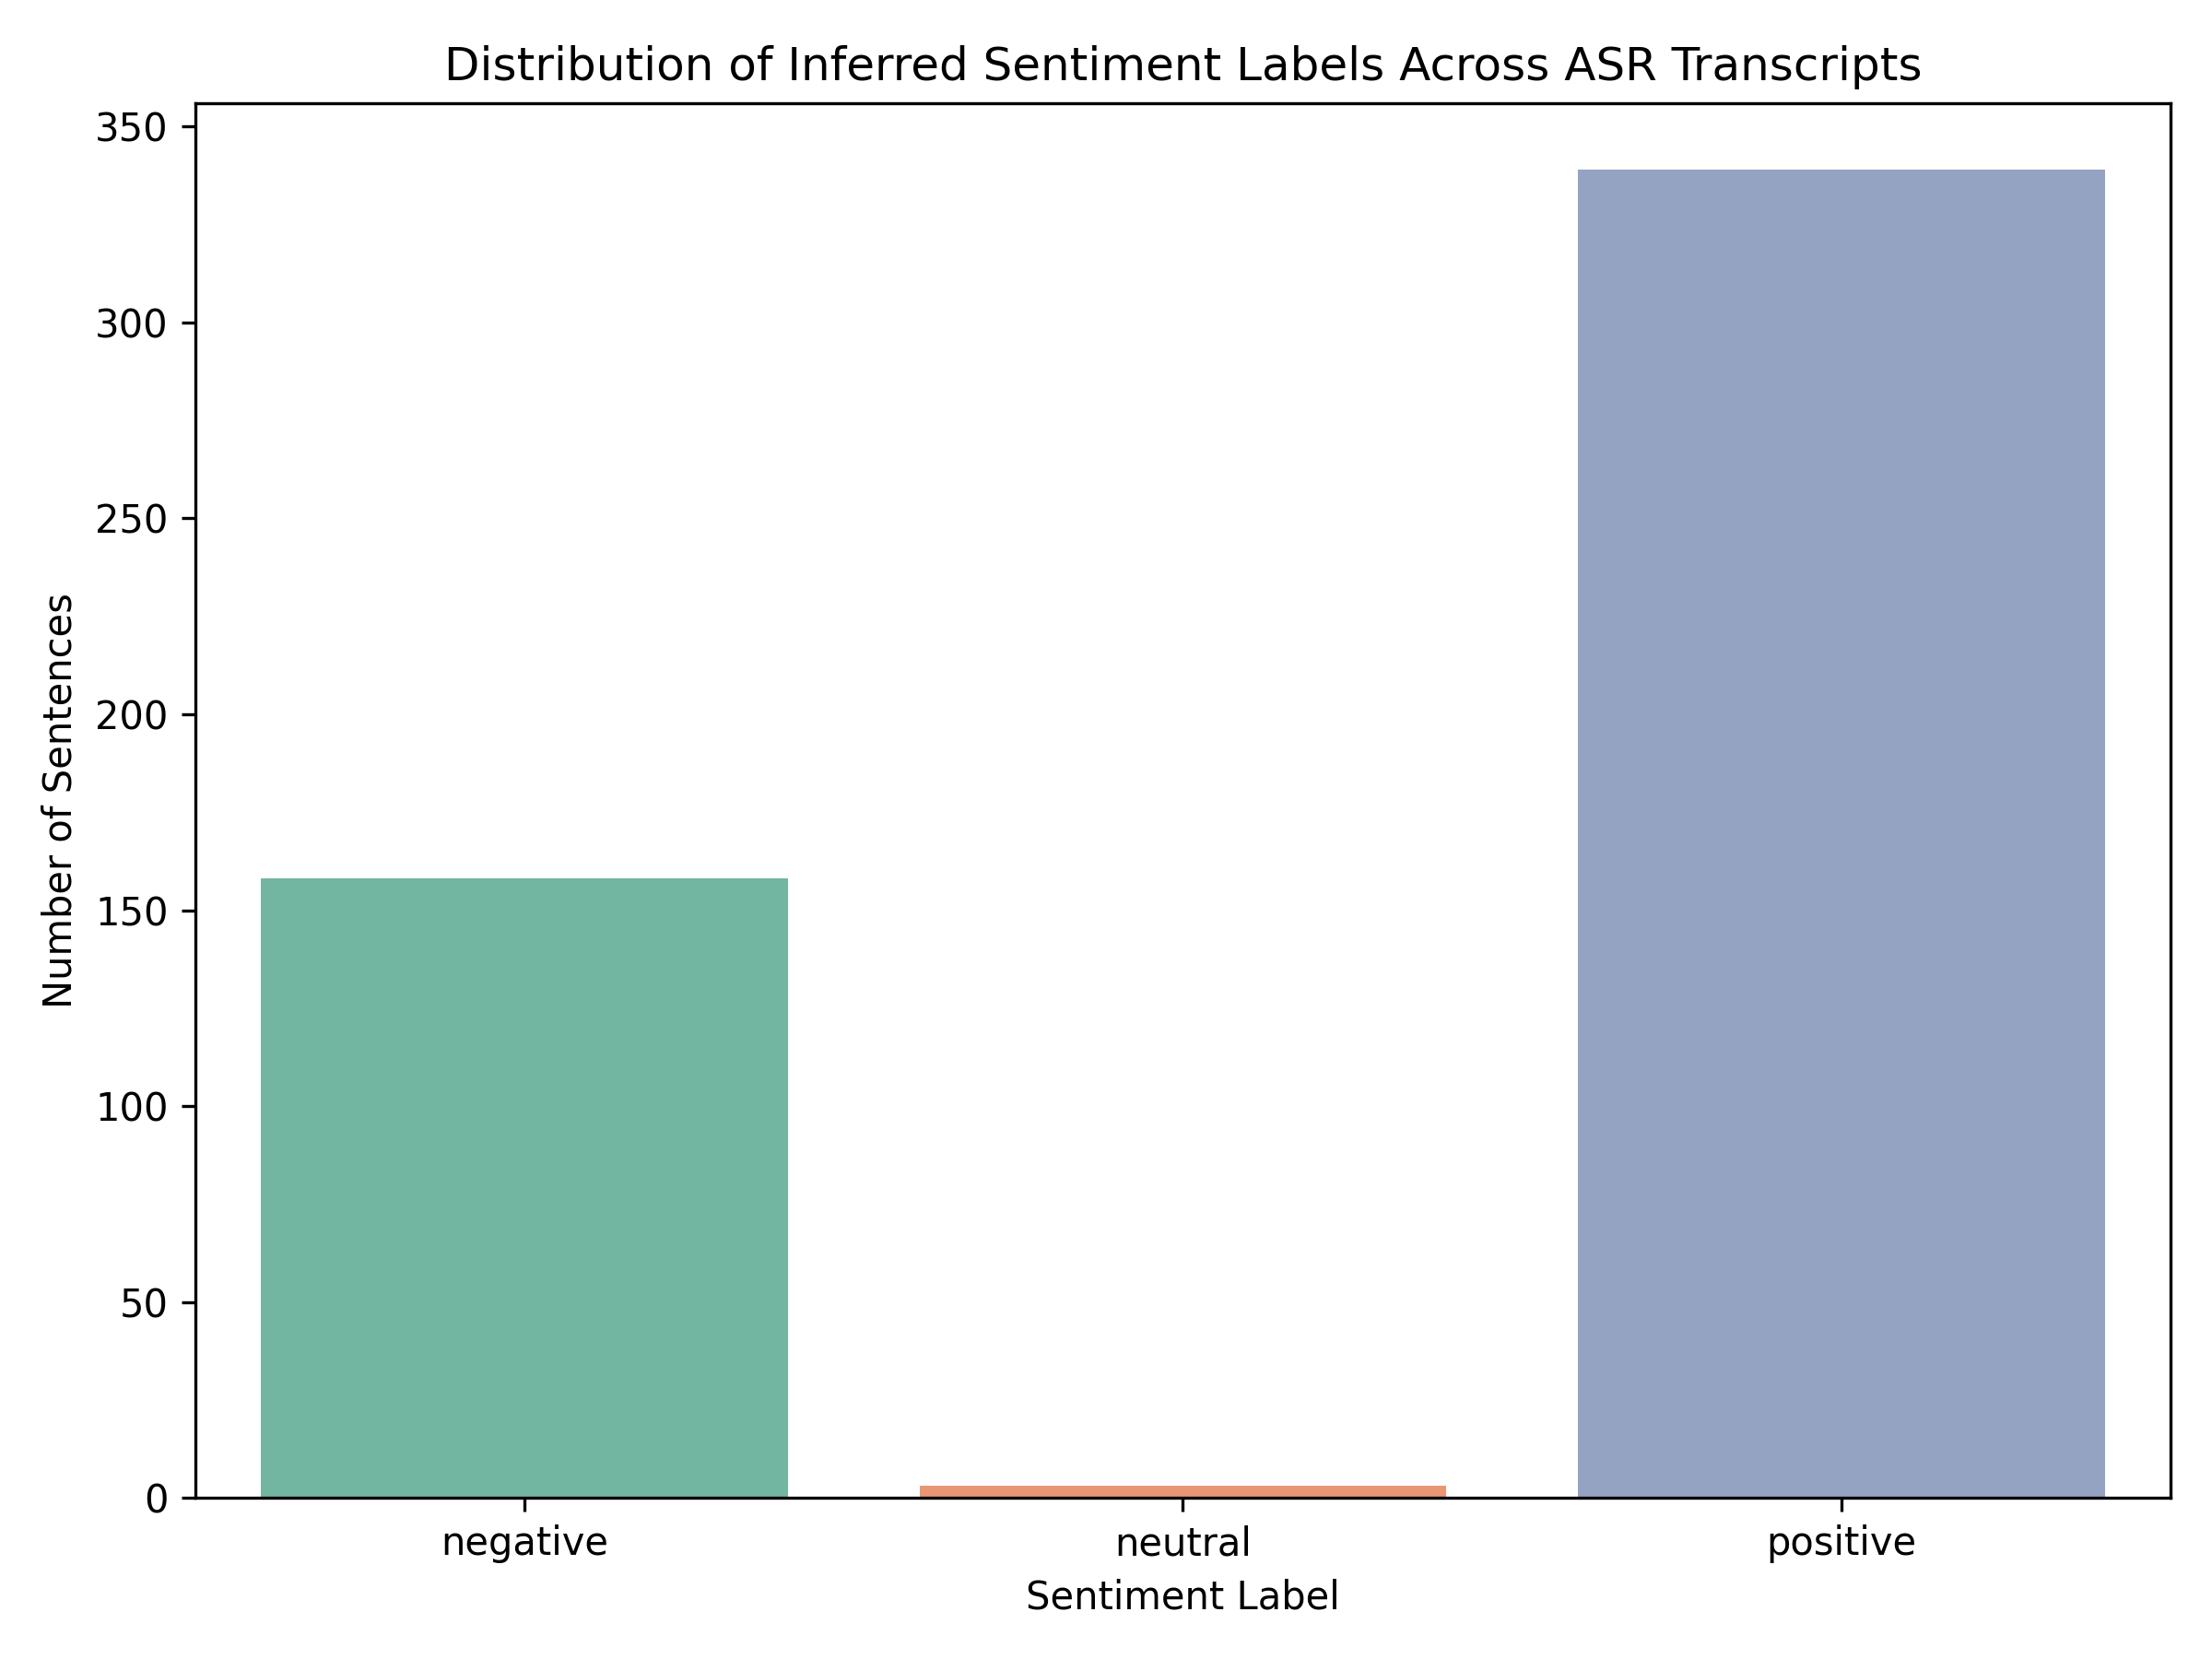
\includegraphics[width=0.75\linewidth]{images/sentiment_distribution.pdf}
    \caption{Distribution of predicted sentiment labels.}
    \label{fig:sentiment_dist}
\end{figure}

% ============================================================
\section*{Summarization Model Evaluation}
\label{app:summarization}

Automatic summarization was evaluated using ROUGE metrics. ROUGE-L is defined as:

\begin{equation}
\text{ROUGE-L} = \frac{\text{LCS}(X, Y)}{|X|}
\end{equation}

where $X$ denotes the reference summary and $Y$ the generated summary. Performance degradation was observed for longer transcripts, motivating the use of chunk-based summarization.

% ============================================================
\section*{System Architecture and Processing Flow}
\label{app:architecture}

The deployed system integrates audio validation, chunking, ASR, text processing, sentiment analysis, summarization, and aggregation into a unified pipeline.

\begin{figure}[h]
    \centering
    \includegraphics[width=0.9\linewidth]{images/processing_flow_architecture.drawio.pdf}
    \caption{End-to-end processing flow architecture of the proposed system.}
    \label{fig:arch}
\end{figure}

% ============================================================
\section*{API Design and JSON Schema}
\label{app:api}

The system exposes a RESTful API implemented using FastAPI. Input and output schemas are validated using Pydantic models to ensure data consistency.

\begin{verbatim}
{
  "transcription": "...",
  "sentiment": "Negative",
  "summary": "...",
  "confidence": 0.87
}
\end{verbatim}

% ============================================================
\section*{Ethical Considerations and Limitations}
\label{app:ethics}

Ethical considerations include demographic bias, cultural misrepresentation in sentiment analysis, and risks of deployment in sensitive contexts. These issues are addressed through transparent reporting, bias analysis, and recommendations for human-in-the-loop deployment.

% ============================================================
\section*{Reproducibility Statement}
\label{app:reproducibility}

All experiments were conducted using fixed random seeds, documented preprocessing scripts, and version-controlled code repositories. Hardware configurations and software dependencies are fully specified to support independent replication.

% ============================================================
% END OF APPENDICES
% ============================================================
